\documentclass{article}
\usepackage{amsmath}
\usepackage{amssymb}
\usepackage{graphicx}
\usepackage{hyperref}
\usepackage[version=4]{mhchem}

\title{Problem 9}
\date{}

\begin{document}
\maketitle

\section*{Problem}
In \(\triangle A B C, \angle B=2 \angle C . A D \perp B C . M\) is the midpoint of \(B C . A B\) is 10 cm . Find the length of \(M D\).\\
\centering
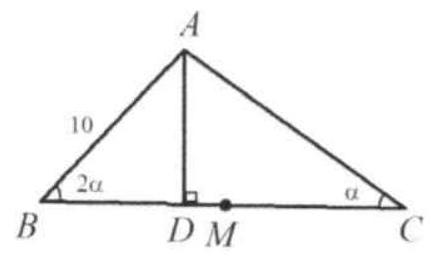
\includegraphics[width=\textwidth]{images/problem_image_1.jpg}

\section*{Solution}
5 cm .
Take \(N\), the midpoint of \(A B\). Connect \(D N, M N\). \(D N\) is the median of right triangle \(A B D\). So \(D N=\frac{1}{2} A B=10 / 2=5, \angle N D B=\angle B=2 \alpha\).\\
\centering
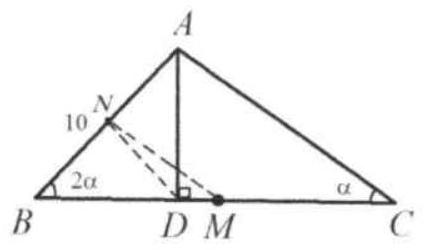
\includegraphics[width=\textwidth]{images/reasoning_image_1.jpg}\\
\(M N\) is the midline of \(\triangle B A C\). So \(M N / / A C\). Thus\\
\(\angle N M B=\angle N M D=\angle C=\alpha\).\\
We know that \(\angle N D B\) is the exterior angle of \(\triangle N D M\). So \(\angle N D B=\angle M N D+\) \(\angle N M D=\angle M N D+\angle \alpha\), or \(\angle M N D+\alpha=2 \alpha \quad \Rightarrow \quad \angle M N D=\alpha\).\\
\(\triangle N M D\) is an isosceles triangle with \(N D=M D=5\).

\end{document}
